% Hand-authored study of where Astra fails on engineering drawings.
% Compile with Tectonic from cvpr2027/:
%   .tools/tectonic docs/latex/eng_frame_failure_study.tex --outdir output/pdf --keep-logs
\PassOptionsToPackage{unicode}{hyperref}
\PassOptionsToPackage{hyphens}{url}
\PassOptionsToPackage{dvipsnames,svgnames,x11names}{xcolor}
\documentclass[11pt,a4paper]{article}
\usepackage{xcolor}
\usepackage[margin=24mm]{geometry}
\usepackage{amsmath,amssymb}
\usepackage{iftex}
\usepackage{lmodern}
\usepackage{textcomp}
\usepackage{parskip}
\usepackage{longtable,booktabs,array}
\usepackage{graphicx}
\usepackage{caption}
\usepackage{enumitem}
\usepackage{float}
\usepackage{needspace}
\usepackage{tikz}
\usepackage{hyperref}
% Shared style; used by generated, standalone LaTeX sources.
\usepackage{xcolor}
\usepackage{xurl}
\usepackage{fvextra}
\usepackage{etoolbox}
\usepackage{fancyhdr}
\usepackage{titlesec}
\definecolor{researchblue}{HTML}{173B58}
\AtBeginDocument{\hypersetup{linkcolor=researchblue,urlcolor=researchblue}}
\pagestyle{fancy}
\fancyhf{}
\fancyhead[L]{\small\sffamily SVG PATCH LAB}
\fancyhead[R]{\small\sffamily CVPR 2027 research package}
\fancyfoot[L]{\small Working documents; results and proposals distinguished}
\fancyfoot[R]{\thepage}
\setlength{\headheight}{15pt}
\setlength{\emergencystretch}{3em}
\titleformat{\section}{\Large\bfseries\color{researchblue}}{\thesection}{0.7em}{}
\titleformat{\subsection}{\large\bfseries\color{researchblue}}{\thesubsection}{0.7em}{}
\DefineVerbatimEnvironment{verbatim}{Verbatim}{breaklines=true,breakanywhere=true,fontsize=\small}
\AtBeginEnvironment{longtable}{\small\setlength{\tabcolsep}{4pt}}
\let\originaltableofcontents\tableofcontents
\renewcommand{\tableofcontents}{\originaltableofcontents\clearpage}

\captionsetup{font=small,labelfont=bf}
\setlist{nosep,leftmargin=1.4em}
\newcommand{\code}[1]{\path{#1}}
\newcolumntype{L}[1]{>{\raggedright\arraybackslash}p{#1}}
\newcolumntype{R}[1]{>{\raggedleft\arraybackslash}p{#1}}
\hypersetup{pdftitle={Where Astra fails on engineering drawings: the EngFrame study},pdfauthor={SVG Patch Lab}}

\title{\color{researchblue}\LARGE Where Astra fails on engineering drawings\\[6pt]
\Large Problem statement, dataset, measured capability boundary and research focus}
\author{SVG Patch Lab \quad\textbullet\quad CVPR 2027 research package\\
\small branch \code{cvpr2027-research-package}\\
\small evidence in \code{runs/eng-frame-*} and \code{runs/eng-frame-aggregate.json}}
\date{22 September 2026}

\begin{document}
\maketitle

\begin{center}
\small\itshape
Status: a measured negative-and-positive result, not a submission. Every number is copied from the
named run artefacts. Declining to answer and answering wrongly are reported as different outcomes
throughout, because only the second puts a false claim on a drawing.
\end{center}

\tableofcontents

% =====================================================================
\section{Executive summary}

On dimensioned structural elevations checked against a frame finite-element reference, GPT-6 Astra
\textbf{declines to produce the required engineering quantities once the frame reaches about twenty
members}, and does so on 4 of 7 samples at that size against 1 of 35 below it (Fisher exact,
two-sided, $p = 0.0015$). It does not fabricate. Across 42 completed samples exactly one reported
quantity fell outside tolerance, and that one did not reproduce on retest.

Three further findings shape how the result should be read.

\begin{enumerate}
\item \textbf{The two failures already recorded in the repository are not reproducible.} The headline
      20 September result --- a peak stress of 179\,MPa against a reference of 20.356\,MPa --- came
      back correct on 3 of 3 fresh samples at the identical protocol. So did the first decline found
      in this study. Single-sample screening manufactures failures that evaporate.
\item \textbf{One apparent model failure was a defect in our own scorer.} Three results were rejected
      for omitting the unit \code{mm} on individual dimension labels, while each drawing declared its
      units once in the notes. That is standard drafting practice, and the harness was penalising
      correct work.
\item \textbf{Accuracy does not decay with complexity; willingness does.} When the model answers, it
      is within tolerance at every size tested, up to 21 members and degree of static indeterminacy 27.
\end{enumerate}

The immediate consequence for the project is that the decline, not the wrong number, is the defect
with a measurable baseline --- and it is precisely the condition a solver-in-the-loop design is meant
to remove.

% =====================================================================
\section{Problem statement}

\subsection{The question}

An engineering drawing is simultaneously a picture and a set of claims. A dimension is an assertion
about a length; a reported stress is an assertion about a solved field. The claims can be false while
the picture stays plausible, and editing the drawing --- moving a grid line, raising a floor, changing
a load --- invalidates every derived claim at once without disturbing the geometry that carries them.

The programme's question is whether a model can produce and edit such drawings so that their numerical
claims remain true, and whether that truth can be \emph{verified} rather than trusted. This study
addresses the narrower empirical precondition:

\begin{quote}
\textbf{On CAD-style engineering drawings whose claims are checkable by simulation, where exactly does
the model stop being reliable, and what does failure look like when it arrives?}
\end{quote}

\subsection{Why engineering drawings specifically}

The artefact under study is a structural elevation of a physical object --- a building frame, a
worktable, a shelf --- emitted as SVG and verified with finite elements. It is deliberately not a
physics field visualisation. An earlier pass in this session built a benchmark on Laplace isotherm
drawings, where a large and robustly reproducible failure does exist; that direction was abandoned
because a contour plot is not an engineering drawing and the reproducible failure there answers a
different question. Section~\ref{sec:abandoned} records it so the effort is not silently lost.

\subsection{What counts as a failure}

A drawing fails when a check that the task explicitly demanded does not hold: a member drawn away from
its centreline, a joint that does not close, a dimension that disagrees with the geometry, a reported
displacement or stress outside tolerance of the reference, or a visible SVG result that contradicts the
returned JSON. Three outcomes are held apart, because the harness conflates them and the distinction
carries the whole finding:

\begin{description}[leftmargin=2.2em,style=nextline]
\item[computed, within tolerance] every checked quantity agrees with the finite-element reference.
\item[computed, outside tolerance] a number was printed on the drawing and it is wrong. This is the
      dangerous case: a released drawing carrying a false engineering claim.
\item[declined] the model returned the contractually permitted \code{status: "unavailable"}, null
      values and a stated reason. The deliverable is incomplete, but no false claim was made.
\end{description}

Truncated responses, API errors and unparseable output are excluded from the denominators rather than
counted as failures.

% =====================================================================
\section{The task and how it is verified}

\subsection{What the model is asked to produce}

Given a physical model in JSON --- nodes, members with rectangular sections $b \times h$, clamped
supports, nodal loads, a probe node --- the model returns one JSON object containing a complete SVG and
an analysis block. The drawing must place every physical member as a single visibly stroked straight
element tagged \code{data-member}, retain member identifiers, honour a fixed \code{viewBox} and a fixed
affine map from millimetres to drawing coordinates, and annotate the centreline length of every member
as text tagged \code{data-dimension}. The analysis must report $u_x$ and $u_y$ at the probe node and the
peak extreme-fibre normal stress
\[
\sigma_{\max} \;=\; \max_{\text{member ends}} \left( \frac{|N|}{A} + \frac{|M|\,h/2}{I} \right),
\]
together with a status of \emph{calculated}, \emph{estimated} or \emph{unavailable}, and must repeat
those three numbers as visible SVG text tagged \code{data-result}. No tools are supplied and the system
prompt forbids claiming that a solver was run. In edit mode the model additionally receives the original
model and its SVG, plus an instruction that changes geometry and a load, and must recompute every
dimension and both analyses.

\subsection{What is checked}

Scoring reuses \code{cad_astra_benchmark.score} unchanged, so results are directly comparable with the
20 September pilot. It parses the SVG with explicit rejection of scripts, stylesheets, clipping, masks,
\code{use} elements and hidden geometry; recovers each tagged member through its accumulated ancestor
transform; and checks member endpoints and straightness to 1\,mm, joint closure to 1\,mm, every
dimension to 1\,mm, the three analysis quantities against the reference at 2\,\% relative tolerance, and
agreement between the JSON numbers and the visible SVG text to 0.1\,\%.

The reference is a linear plane-frame finite-element solution --- axial plus Euler--Bernoulli bending,
rigid joints, small displacements, nodal loads --- assembled independently of the model's output.

% =====================================================================
\section{Dataset: EngFrame}

\subsection{Design principle: order the family by static indeterminacy}

The pilot contained three hand-built families and exactly one failure. Ordering them by degree of static
indeterminacy for a plane frame,
\[
i \;=\; 3m + r - 3j,
\]
with $m$ members, $r$ reaction components and $j$ joints, reproduces their outcomes exactly:

\begin{center}
\begin{tabular}{lccl}
\toprule
Pilot family & Members & $i$ & Pilot outcome \\
\midrule
shelf (cantilever chain) & 4 & 0 & pass \\
table (portal frame) & 4 & 3 & pass \\
building (two-storey setback) & 8 & 9 & the sole failure \\
\bottomrule
\end{tabular}
\end{center}

The axis is mechanically meaningful rather than fitted after the fact: a determinate frame ($i = 0$)
is solvable by statics alone, whereas an indeterminate one requires the simultaneous stiffness system,
which is what must be carried out without a solver. EngFrame generates frames along that axis.

\subsection{The generator}

\code{scripts/eng_frame_bench.py} builds fixed-base rectilinear building frames from a small parameter
set: number of bays, number of storeys, bay width, storey height, and an optional setback that removes
the rightmost column lines above a chosen floor --- the shape of the pilot's two-storey building. Column
and beam sections thin with height. Loads are applied at the outer nodes of every floor. For a plain
rectangular fixed-base frame with $n_b$ bays and $n_s$ storeys the construction gives $i = 3\,n_b n_s$
exactly, so the difficulty axis is controlled by construction rather than measured after generation.

Each family is emitted twice, in \emph{generate} and \emph{edit} mode, where the edit shifts a column
grid by 700\,mm or raises the top floor by 600\,mm and changes a nodal load by 15\,kN. Verification
requires that every edit changes both the dimensions and all three analysis quantities, so that no
instance can be satisfied by copying the source.

\subsection{Reference certification}

A reference is admitted only if it survives two independent checks: member-subdivision invariance,
requiring the nodal response with each member split into four elements to agree with the single-element
assembly to a relative $10^{-7}$; and global force and moment equilibrium, requiring the residual to be
below $10^{-9}$ of the largest applied load component. Eight further manifest checks pass, among them
that every frame is well formed with its recorded indeterminacy correct, that every reference design
satisfies its own stated limits, and --- the positive control --- that the harness scores a drawing
constructed from the reference itself as a pass.

\subsection{Composition}

Instances are concentrated in the hard region on purpose. There is no value in re-measuring the region
the model already solves, so 14 of the 18 main instances sit at $i \geq 9$, with a separate extension
set at $i = 24$ and $27$. The extension set deliberately carries no control; its manifest records that
controls live in the companion main set, and verification enforces that pairing rather than waiving it.

\begin{center}
\begin{tabular}{lrrrrr}
\toprule
Family & Members & Nodes & Supports & $i$ & Reference $\sigma_{\max}$ (MPa) \\
\midrule
\multicolumn{6}{l}{\itshape Main set --- 9 families, 18 tasks} \\
control\_portal & 3 & 4 & 2 & 3 & 9.550 \\
control\_twobay & 5 & 6 & 3 & 6 & 6.233 \\
setback\_a & 8 & 8 & 3 & 9 & 14.934 \\
setback\_b & 8 & 8 & 3 & 9 & 15.829 \\
threestorey & 9 & 8 & 2 & 9 & 33.540 \\
twostorey\_a & 10 & 9 & 3 & 12 & 13.863 \\
twostorey\_b & 10 & 9 & 3 & 12 & 13.215 \\
setback\_tall & 13 & 12 & 4 & 15 & 31.616 \\
threebay & 14 & 12 & 4 & 18 & 10.860 \\
\midrule
\multicolumn{6}{l}{\itshape Extension set --- 3 families, 6 tasks} \\
fourbay & 18 & 15 & 5 & 24 & 9.110 \\
twobay\_four & 20 & 15 & 3 & 24 & 33.316 \\
threebay\_three & 21 & 16 & 4 & 27 & 17.185 \\
\bottomrule
\end{tabular}
\end{center}

% =====================================================================
\section{What Astra cannot do}
\label{sec:cannot}

\subsection{The boundary}

Forty-five samples were collected, of which 42 completed; the remaining three were cut off by credit
exhaustion and are excluded. Outcomes group sharply by frame size.

\begin{center}
\begin{tabular}{rrrrrr}
\toprule
Members & Samples & Correct & Outside tolerance & Declined & Decline rate \\
\midrule
3--13 & 25 & 25 & 0 & 0 & 0\,\% \\
14 & 8 & 7 & 0 & 1 & 12\,\% \\
18 & 2 & 2 & 0 & 0 & 0\,\% \\
20 & 2 & 1 & 0 & 1 & 50\,\% \\
21 & 5 & 2 & 0 & 3 & 60\,\% \\
\midrule
\textbf{$<$ 20} & \textbf{35} & 34 & 1 & \textbf{1} & \textbf{3\,\%} \\
\textbf{$\geq$ 20} & \textbf{7} & 3 & 0 & \textbf{4} & \textbf{57\,\%} \\
\bottomrule
\end{tabular}
\end{center}

The contrast between the two pooled rows is significant at $p = 0.0015$ by a two-sided Fisher exact
test. The decline rate above the boundary is 57\,\% with a 95\,\% Wilson interval of 25--84\,\%.

\begin{figure}[H]
\centering
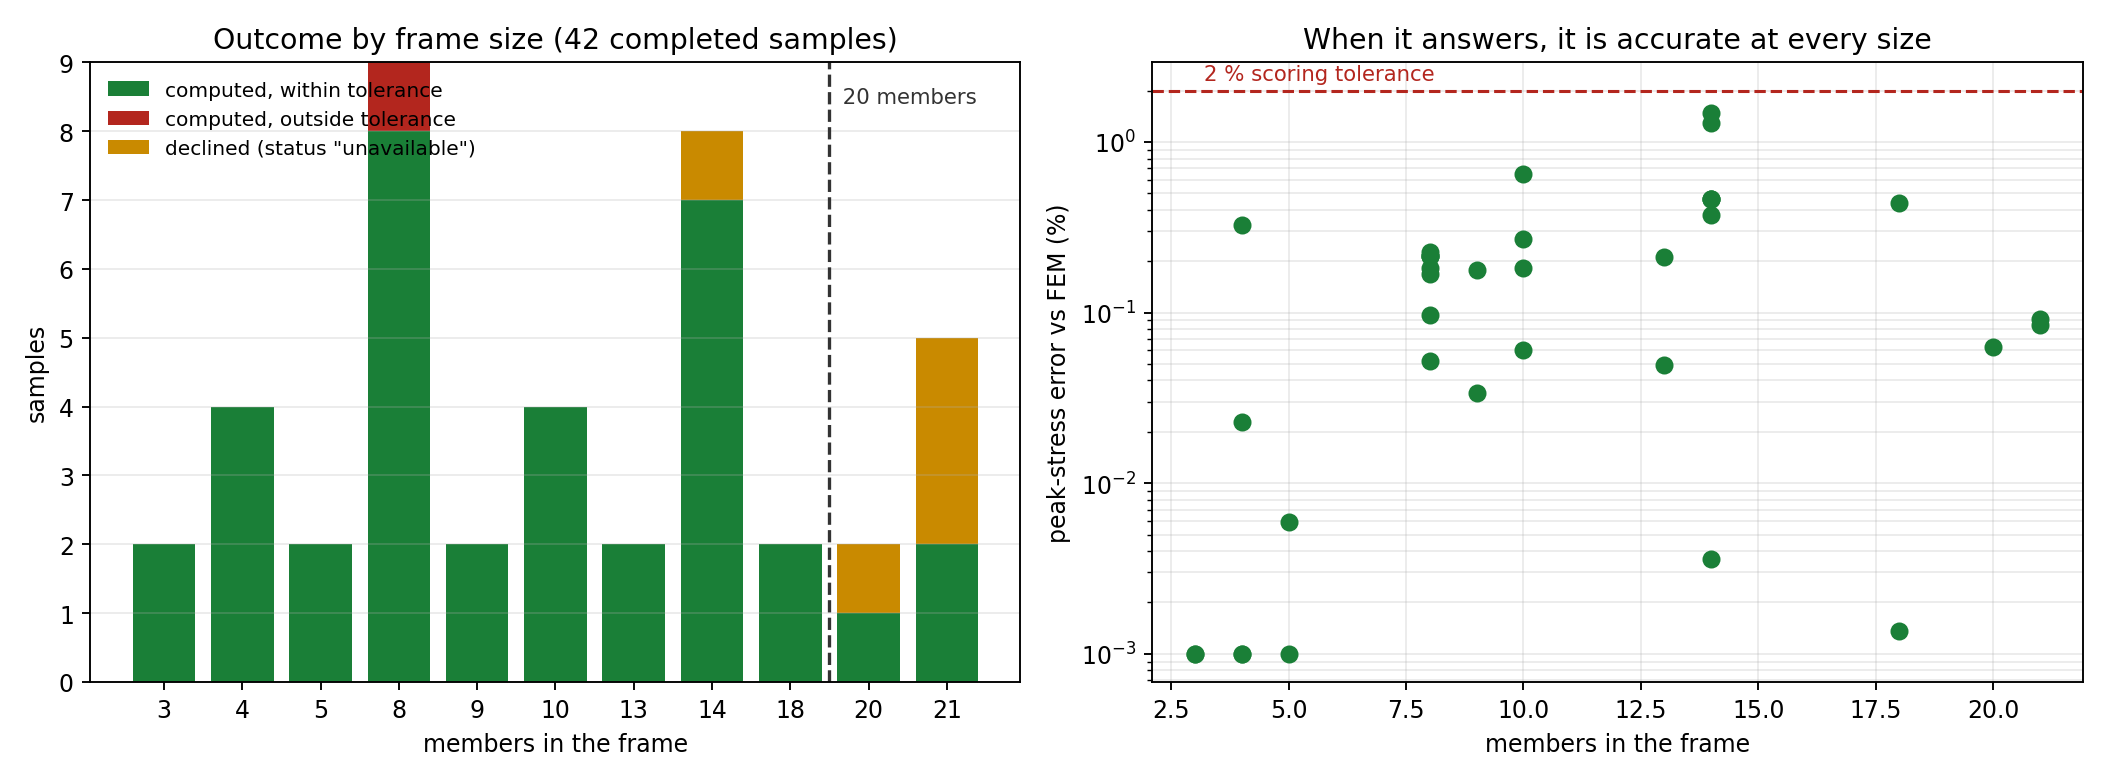
\includegraphics[width=\textwidth]{../../paper/figures/eng_frame_results.png}
\caption{Left: outcome by frame size across 42 completed samples; declines appear only at the top of
the range. Right: for every sample where a number was given, its peak-stress error against the
finite-element reference. All 36 lie below the 2\,\% tolerance and show no trend with size.}
\end{figure}

\subsection{What the failure looks like}

The declines are explicit and honest. The model sets the permitted status, returns nulls, and states a
specific reason --- for the 21-member edit, \emph{``the edited frame stiffness solution and member-end
force recovery have not been performed''}; for the 20-member generation, \emph{``the coupled
axial--bending frame response has not been computed''}. It identifies precisely the step it did not
carry out. Token budget is not the constraint: declines finish cleanly with \code{finish_reason=stop}
after 6{,}600--8{,}100 completion tokens against a 32{,}000 cap, while successful answers on the same
instances use 9{,}000--13{,}000.

This is a capability boundary in \emph{willingness to carry out an unaided indeterminate solve}, not in
drafting. In every declining sample the geometry and the dimensions were still produced.

\subsection{What it can do, for scope}

The claim must be bounded by an equally clear statement of competence. Across this study the model drew
every frame correctly, at every size, in both modes. When it reported numbers they were within tolerance
in all 36 cases, including at 21 members and $i = 27$, where it returned a peak stress of 17.7\,MPa
against a reference of 17.6837 and $u_x$ of 3.5 against 3.5119. On the pilot's failing instance it had
already identified the correct governing member end and stated the correct extreme-fibre formula. Prior
work in this package further records that the model solves PCB routing with clearance and exact-length
constraints, irregular part nesting, multiview machining edits and FEM-constrained section sizing. The
honest summary is that this task family is close to solved, with one measurable exception.

% =====================================================================
\section{Negative results and two corrections}

\subsection{Recorded failures that did not reproduce}

\begin{center}
\begin{tabular}{L{4.6cm}L{5.4cm}L{4.4cm}}
\toprule
Lead & Recorded result & On retest at identical protocol \\
\midrule
\code{building_edit}, 20 Sep pilot & peak stress 179\,MPa against a reference of 20.356\,MPa & 3 of 3 samples correct (20.4\,MPa) \\
\code{threebay_edit}, this study & analysis declined & 3 of 3 samples correct \\
\bottomrule
\end{tabular}
\end{center}

The 179\,MPa case remains the most diagnostic artefact in the repository. Geometry and dimensions were
correct, both displacements were right to 0.3\,\%, the governing member end was correctly named, and the
formula was correctly stated --- and the number printed was 8.8 times too large. It is a genuine defect
and it is not reproducible, so under the pilot's own admission rule it is not an Astra-hard case and must
not be cited as one.

\subsection{A harness defect mistaken for a model defect}

Three screened results were filed as unscored format failures for ``missing mm unit'' on every dimension
label. Inspection shows each drawing declares its units once, for instance \emph{``Structural elevation
$\cdot$ dimensions in mm $\cdot$ member centrelines''}. Stating units once in the notes rather than
repeating them on every dimension is standard ISO and ASME practice, so the harness was rejecting correct
drafting. \code{eng_frame_bench.adjudicate} withdraws that complaint, but only when the drawing declares
its units and nothing else fails; it can never convert a failure into a pass on any other ground. One of
those three, \code{twobay_four_generate}, proved to have declined its analysis as well --- the unit
complaint had masked the real defect.

\subsection{Methodological consequence}

Three of the first four anomalies found in this study disappeared on repetition. Any screen reporting
one sample per task will therefore report failures that do not exist, and --- since a 57\,\% decline rate
still yields a pass 43\,\% of the time --- will also miss real ones. Confirmation at three or more fresh
samples is not bureaucratic caution here; it is the difference between the two headline leads being real
and being noise. Both were noise.

% =====================================================================
\section{Our focus}

\subsection{The immediate experiment}

The decline is the right target, for three reasons. It is statistically established rather than
anecdotal; it is the only measured boundary in a family the model otherwise solves; and it is exactly
the condition that the project's solver-in-the-loop thesis predicts should be removable. The experiment
is direct: re-run the instances at and above 20 members with a numerical tool available --- a stiffness
solve or member-end force recovery the model may call --- and measure whether the decline rate falls
while accuracy is preserved. A baseline of 4 declines in 7 samples now exists to measure against.

Two secondary arms follow cheaply: raising the reasoning effort and the token cap at fixed tool access,
to separate unwillingness from budget; and extending the ladder beyond 21 members to locate the
threshold, which the present data brackets only loosely between 18 and 20.

\subsection{Why this reframes the project's premise}

The programme was organised around the hypothesis that the model would draw plausibly and be
\emph{numerically wrong}, so that binding claims to a verified solution would catch silent errors. The
measurement does not support that in this family. The model is numerically right whenever it commits,
and when it cannot commit it says so. The valuable contract is therefore not primarily a lie detector
but a \emph{completion} mechanism: the verification layer supplies the solve the model declines to
attempt, and the drawing is finished rather than rejected. That is a narrower and better-evidenced
claim than the original framing, and it is the one the artefacts here support.

The one recorded instance of a confidently wrong number, at 1 in 42 samples, keeps the verification
argument alive but cannot carry it alone; establishing that rate would need roughly an order of
magnitude more samples than this study could fund.

\subsection{Relation to existing work}

Combining a language model, a simulator and vector graphics is not novel, and the package's prior-art
review already records close precedents: EngDesign for functionally simulated design tasks,
StructureClaw for linked structural artefacts with numerical checks, ALL-FEM for fine-tuned solver-code
agents, PDEAgent-Bench for calibrated PDE references, and SSVG-Bench for structured scientific vector
graphics. What this study contributes is narrower and empirical: a procedurally generated engineering
drawing family ordered by a mechanically meaningful difficulty parameter, with certified references, and
a measured capability boundary with its statistics and its non-reproducing counterexamples stated. That
is a benchmark and a measurement, not a method claim.

\subsection{The abandoned direction}
\label{sec:abandoned}

A benchmark on Laplace isotherm drawings over procedurally generated rectilinear plates was built and
verified before being set aside as off-target. It is retained because its findings are independently
useful: the generator reproduces the 18 September failing task character for character; the worst grid
sensitivity of the finite-difference reference sits exactly on the re-entrant corners, which therefore
must be excluded from any scored metric; and the strict criterion used on 18 September is unreachable on
that domain, since a drawing built from the reference isolines themselves scores 5.0003 percentage points
against a 0.5 point tolerance. The 90.0 point maxima reported there are that artefact, not a finding.
Artefacts are in \code{data/polyheat-bench/} with 15 passing tests.

% =====================================================================
\section{Limits}

Seven completed samples above the boundary is a small denominator, and the 25--84\,\% interval is
correspondingly wide. The threshold is bracketed, not resolved: 18 members passed twice, 20 and 21
declined in 4 of 7 samples, so ``about twenty members'' is the defensible statement and the confound
between member count and degree of indeterminacy is not separated by these data. The
\code{twobay_four_generate} confirmation was cut off by credit exhaustion, leaving that instance with a
single screened sample; its three attempts are recorded as excluded API errors and the runner will not
re-bill them, so completing it requires a fresh output directory.

All runs used \code{gpt-6-astra} at medium reasoning effort through Chat Completions with
\code{store=false}. Whether a larger budget, higher effort or tool access removes the decline is untested.
The structural model is linear, planar, rigid-jointed and small-displacement with nodal loads and
rectangular sections; self-weight, shear deformation, buckling, out-of-plane behaviour, connection
flexibility and code compliance are all outside it. The scoring is a geometric and numerical audit of
tagged elements, not a rendered-image review: occlusion, legibility, line weights, layer conventions and
title-block practice are not assessed. Nothing here bounds performance on 3D CAD or on drawing families
other than planar frame elevations.

% =====================================================================
\section{Artefacts and reproduction}

\begin{center}
\begin{tabular}{L{6.2cm}L{8.4cm}}
\toprule
Path & Contents \\
\midrule
\code{scripts/eng_frame_bench.py} & generator, reference certification, 8 verification checks, units adjudication \\
\code{scripts/eng_frame_report.py} & cross-run aggregation separating declined from wrong \\
\code{data/eng-frame-bench/} & main set, 18 tasks, $i = 3$--18 \\
\code{data/eng-frame-bench-xl/} & extension set, 6 tasks, $i = 24$--27 \\
\code{runs/eng-frame-*/} & screens, confirmations, per-sample requests and responses \\
\code{runs/eng-frame-aggregate.json} & the 45-sample table behind every figure here \\
\code{reports/ENG_FRAME_FAILURE_BOUNDARY_20260922.md} & the prose record \\
\bottomrule
\end{tabular}
\end{center}

\begin{verbatim}
cd cvpr2027
PYTHONPATH=src ../.venv/bin/python scripts/eng_frame_bench.py build
PYTHONPATH=src ../.venv/bin/python scripts/eng_frame_bench.py build --set xl \
    --data data/eng-frame-bench-xl
PYTHONPATH=src ../.venv/bin/python scripts/eng_frame_bench.py verify
PYTHONPATH=src ../.venv/bin/python scripts/cad_astra_benchmark.py run   \
    --data data/eng-frame-bench --output runs/<fresh> --samples 3      # billable
PYTHONPATH=src ../.venv/bin/python scripts/cad_astra_benchmark.py score \
    --data data/eng-frame-bench --output runs/<fresh>
PYTHONPATH=src ../.venv/bin/python scripts/eng_frame_bench.py adjudicate --output runs/<fresh>
PYTHONPATH=src ../.venv/bin/python scripts/eng_frame_report.py
\end{verbatim}

\code{build} is deterministic. \code{run} resumes without re-billing a sample whose result exists, and
refuses a directory created under a different protocol.

% =====================================================================
\section{Provenance and cost}

This study used 115{,}455 input and 375{,}052 completion tokens, approximately \textbf{\$19.91} at the
documented list prices of \$10 and \$50 per million tokens. That is token-price arithmetic, not an
invoice or a balance reading. Of it, \$1.18 went to the abandoned isotherm direction and \$0.87 to a void
run whose prompts omitted the \code{data-level} contract and which is retained, clearly marked, at
\code{runs/VOID-polyheat-zeroshot-20260922-missing-status-line/}. The account returned
\code{credit_balance_exhausted} during the final confirmation, which is why one instance remains
incomplete.

All model outputs, requests, protocols and scores are retained unmodified. Where a verdict was changed
after the fact --- only the withdrawal of per-label unit complaints --- the original score, the new score
and the reason are stored side by side in the run's \code{adjudication.json}.

\end{document}
